\documentclass[a4j]{ujarticle}
% \documentclass[a4j]{jarticle}
\renewcommand{\baselinestretch}{0.85}
\usepackage[top=1.5cm, bottom=1.5cm, left=1.5cm, right=1.5cm]{geometry}
\usepackage{xcolor}
\usepackage[dvipdfmx]{graphicx, hyperref}
\usepackage{listings}
\usepackage{multirow}
\usepackage{siunitx}
\usepackage{subfig}
\usepackage{url}
\usepackage{listings}

\colorlet{punct}{red!60!black}
\definecolor{background}{HTML}{EEEEEE}
\definecolor{delim}{RGB}{20,105,176}
\colorlet{numb}{magenta!60!black}

\newcommand{\Sref}[1]{\mbox{\ref{sec:#1}}}
\newcommand{\Tref}[1]{\mbox{表\ref{tab:#1}}}
\newcommand{\Eref}[1]{\mbox{式(\ref{eq:#1})}}
\newcommand{\Fref}[1]{\mbox{図\ref{fig:#1}}}
\renewcommand{\lstlistingname}{ソースコード}
\newcommand{\Lref}[1]{\mbox{ソースコード\ref{lst:#1}}}
\newcommand{\bhline}[1]{\noalign{\hrule height #1}}

\lstdefinelanguage{json}
{
    basicstyle=\normalfont\ttfamily,
    numbers=left,
    numberstyle=\scriptsize,
    stepnumber=1,
    numbersep=8pt,
    showstringspaces=false,
    breaklines=true,
    backgroundcolor=\color{background},
    literate=
     *{:}{{{\color{punct}{:}}}}{1}
      {,}{{{\color{punct}{,}}}}{1}
      {\{}{{{\color{delim}{\{}}}}{1}
      {\}}{{{\color{delim}{\}}}}}{1}
      {[}{{{\color{delim}{[}}}}{1}
      {]}{{{\color{delim}{]}}}}{1},
}
\lstset{
	frame=tRBl,
	captionpos=b,
	numbers=left,
	tabsize=4,
    columns=[l]{fullflexible},
    breaklines=true,
}

\hypersetup{
	setpagesize=false,
	bookmarksnumbered=true,
	bookmarksopen=true,
	colorlinks=true,
	linkcolor=black,
	citecolor=black
}

\begin{document}

	\begin{flushright}
		MDLab GM資料\\
		21年10月26日(火)
	\end{flushright}

	\begin{center}
		{\Large	腹部超音波画像からの腫瘍検出}
	\end{center}

	\begin{flushright}
		{\large B3  原 英吾}\\
	\end{flushright}

	\section{研究背景および目的}
		\begin{figure}[h]
			\begin{minipage}{.59\textwidth}
				\begin{itemize}
					\item 背景
					\begin{itemize}
						\item 検査実施者は超音波器具の操作と同時に診断を行わなければならず高難易度
						\item 肝臓は沈黙の臓器と呼ばれ,炎症やガンがあっても初期には自覚症状がほとんどない
						\begin{itemize}
							\item 症状を自覚しているときには重症化しているケースが多い
						\end{itemize}
						\item 機械学習による診断のサポート
						\begin{itemize}
							\item 提供されているデータセットには,\Fref{ex}の様に明らかなアノテーション不足のある画像が存在する
						\end{itemize}
					\end{itemize}
					\item 目的
					\begin{itemize}
						\item 既存の研究を踏まえたモデルの精度向上
						\begin{itemize}
							\item noisy label\footnotemark[1]による精度低下の改善
						\end{itemize}
						\item 超音波支援システムの開発
						\begin{itemize}
							\item 早期発見につながると良い
						\end{itemize}
					\end{itemize}
				\end{itemize}
			\end{minipage}
			\begin{minipage}{.39\textwidth}
				\centering
				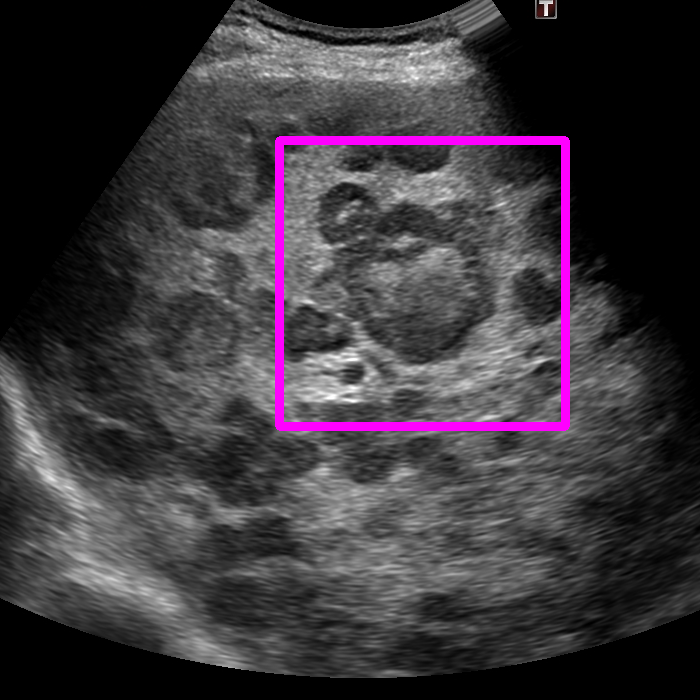
\includegraphics[width=.9\linewidth]{../fig/pseudo.png}
				\caption{アノテーション不足のある診断画像例}
				\label{fig:ex}
			\end{minipage}
		\end{figure}

\footnotetext[1]{今回は\Fref{ex}の様なアノテーションが不足しているものを指す}
\addtocounter{footnote}{1}

	\section{これまでの研究のまとめ}
		\begin{itemize}
			\item データセット
			\begin{itemize}
				\item 国立研究開発法人日本医療研究開発機構(AMED)\footnote{\url{https://www.amed.go.jp/}}が提供している延べ8万人に及ぶ以下のデータが付随
				\begin{itemize}
					\item 腹部超音波画像,ROI
					\item 年齢,性別
				\end{itemize}
			\end{itemize}

			\begin{figure}[ht]
				\begin{minipage}{.59\textwidth}
					\begin{itemize}
						\item 性別毎の画像枚数の分布(\Fref{sex})
						\begin{itemize}
							\item hemangioma (血管腫)
							\begin{itemize}
								\item 肝臓にできる良性腫瘍の中で最も多い\footnotemark[4]
								\item 女性ホルモンが原因が原因で女性が罹患しやすいと言われているが詳しくは解明されていない\footnotemark[7]
							\end{itemize}
							\item hcc (肝細胞癌)
							\begin{itemize}
								\item 肝臓にできる悪性腫瘍の中で最も多いと言われている\footnotemark[4]
								\item 昔は男性の方が飲酒・タバコが多く癌に罹りやすかったという時代背景があるかもしれない
							\end{itemize}
							\item meta (転移性肝癌)
						\end{itemize}
					\end{itemize}
				\end{minipage}
				\begin{minipage}{.39\textwidth}
					\centering
					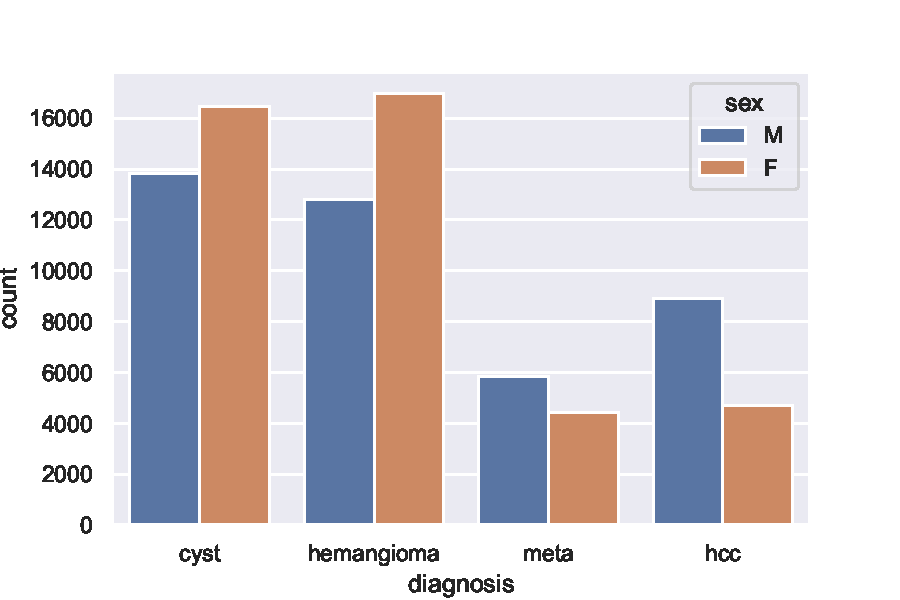
\includegraphics[width=\linewidth]{../fig/sex_a.pdf}
					\caption{性別毎の画像枚数}
					\label{fig:sex}
				\end{minipage}
			\end{figure}

			\begin{figure}[ht]
				\begin{minipage}{.59\textwidth}
					\begin{itemize}
						\item 年齢の分布(\Fref{age})
						\begin{itemize}
							\item hcc(肝細胞癌)は比較的高齢者が罹患しやすい
							\item cyst(単純嚢胞),hemangioma(血管腫)の分布にははあまり特徴がない
							\item meta(転移性肝癌)における0歳はラベルミスである可能性が高い
						\end{itemize}
					\end{itemize}
				\end{minipage}
				\begin{minipage}{.39\textwidth}
					\centering
					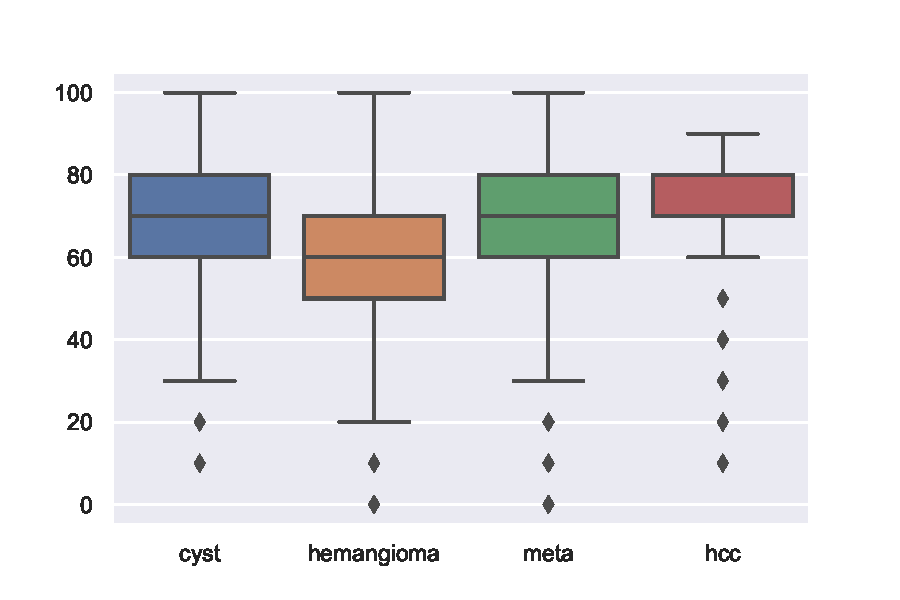
\includegraphics[width=\linewidth]{../fig/age_a.pdf}
					\caption{診断名毎の年齢分布}
					\label{fig:age}
				\end{minipage}
			\end{figure}
			\begin{figure}[ht]
				\begin{minipage}{.59\textwidth}
					\begin{itemize}
						\item 画像サイズの分布(\Fref{area})
						\begin{itemize}
							\item hemangioma(血管腫)は比較的画像サイズが統一されていることが読み取れる
							\begin{itemize}
								\item 血管腫においては腫瘍の大きさが血管に依存するためあまり偏りが生じていない?
							\end{itemize}
						\end{itemize}
					\end{itemize}
				\end{minipage}
				\begin{minipage}{.39\textwidth}
					\centering
					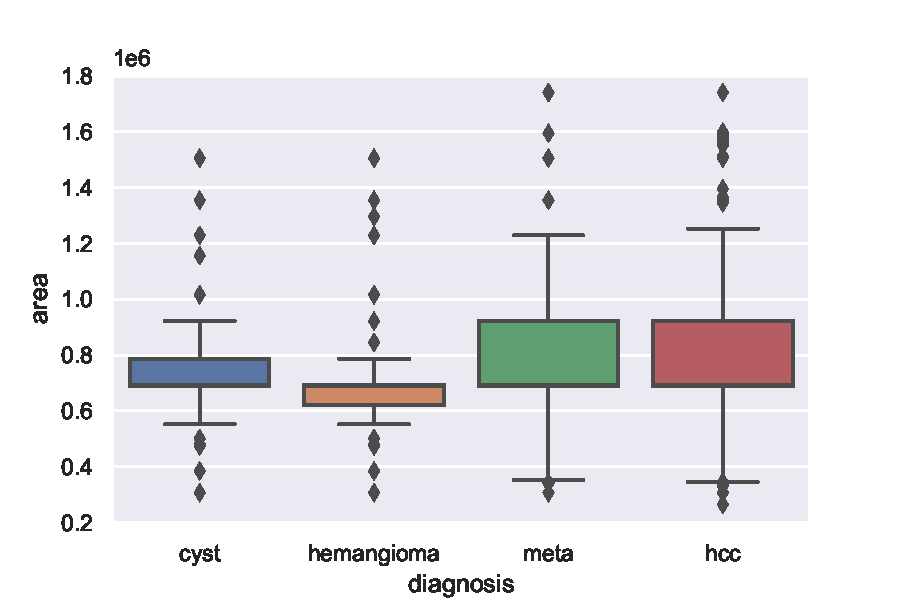
\includegraphics[width=\linewidth]{../fig/area_a.pdf}
					\caption{画像サイズ$(h \times w)$の分布}
					\label{fig:area}
				\end{minipage}
			\end{figure}
			\begin{figure}[ht]
				\begin{minipage}{.59\textwidth}
					\begin{itemize}
						\item 画像サイズの分布(\Fref{ratio})
						\begin{itemize}
							\item cyst(単純嚢胞)は他の診断と比べてbboxの割合が低い($\frac{1}{2}$程度)であることが読み取れる
						\end{itemize}
					\end{itemize}
				\end{minipage}
				\begin{minipage}{.39\textwidth}
					\centering
					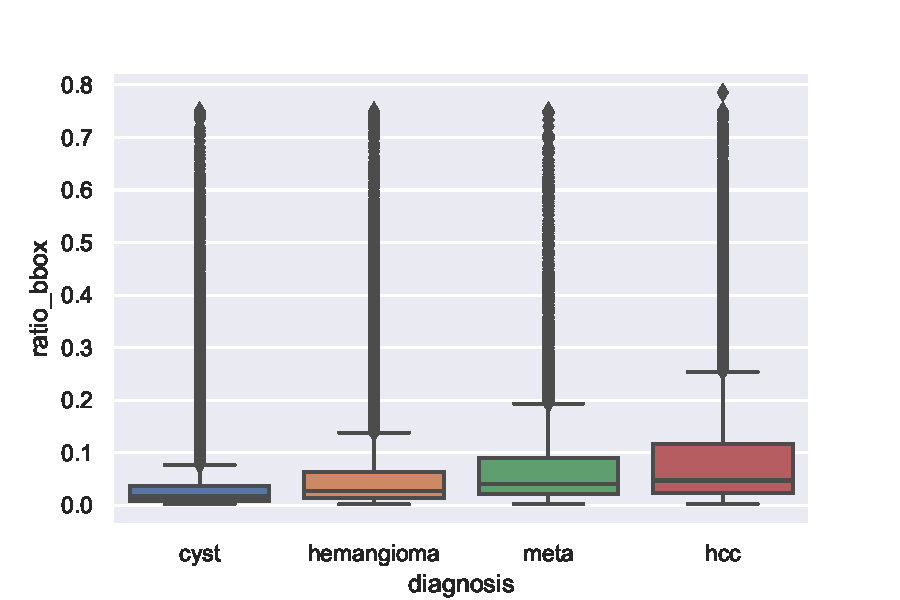
\includegraphics[width=\linewidth]{../fig/ratio_bbox_a.pdf}
					\caption{画像サイズ$(h \times w)$の分布}
					\label{fig:ratio}
				\end{minipage}
			\end{figure}
		\end{itemize}

\clearpage

	\section{前回のGMからの進捗}
		\begin{itemize}
			\item 症状毎の特徴について調査
				\begin{itemize}
					\begin{figure}[ht]
						\begin{minipage}{.79\linewidth}
							\item cyst (単純嚢胞)\footnotemark[3]
							\begin{itemize}
								\item 液体が貯留されている状態
								\item 症状がでないことが多いことから大きな腫瘍になって発見されることが多い
								\item 嚢胞の内腔に向けて増殖するため転移することは少ない
							\end{itemize}
						\end{minipage}
						\begin{minipage}{.09\linewidth}
							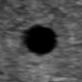
\includegraphics[width=\linewidth]{../fig/cyst.jpg} \caption{cyst} \label{fig:cyst}
						\end{minipage}
					\end{figure}
					% \begin{figure}
					% 	\begin{minipage}{width=.79\linewidth}
					% 		\item hemangioma (血管腫)\footnotemark[4]
					% 			\begin{itemize}
					% 				\item 血管が無数に絡み合うことによって出来た血管の塊であることから血流が遅いという特徴がある
					% 				\item 他の臓器に浸潤したり転移することは無いと言われている
					% 			\end{itemize}
					% 			\item meta (転移性肝癌)
					% 			\begin{itemize}
					% 				\item 門脈\footnotemark[5]を介して大腸癌などの消化器癌から転移する割合が多い
					% 				\item 類似したエコーパターンをもつ腫瘤が多発してみられることが多い\footnotemark[6]
					% 			\end{itemize}
					% 			\item hcc (肝細胞癌)
					% 			\begin{itemize}
					% 				\item 約90%がウイルス感染症が原因\footnotemark[4]
					% 			\end{itemize}
					% 	\end{minipage}
					% 	\begin{minipage}{width=0.19\linewidth}
					% 		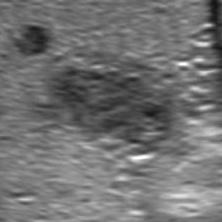
\includegraphics[width=\linewidth]{../fig/hemangioma.jpg}
					% 	\end{minipage}
					% \end{figure}
				\end{itemize}
		\end{itemize}

\clearpage

	\begin{thebibliography}{9} 
		\bibitem{recognition} Jingdong Wang, Ke Sun, Tianheng Cheng, Borui Jiang, Chaorui Deng, Yang Zhao, Dong Liu, Yadong Mu, Mingkui Tan, Xinggang Wang, Wenyu Liu, and Bin Xiao. \href{https://arxiv.org/pdf/1908.07919.pdf}{Deep High-Resolution Representation Learning for Visual Recognition}, 2020.
		\bibitem{cleanlab} Curtis G. Northcutt, Lu Jiang, and Isaac L. Chuang. \href{https://arxiv.org/pdf/1911.00068.pdf}{Confident Learning: Estimating Uncertainty in Dataset Labels}, 2021.
	\end{thebibliography}
\end{document}
